\subsection{Dyscalculia}

Dyscalculia is a learning disorder that primarily affects a child's ability to understand and work with numbers. Individuals with dyscalculia often encounter challenges in basic arithmetic operations, number sense, and mathematical reasoning. To develop effective interventions for children with dyscalculia, it is crucial to understand their unique user profile. This includes identifying their specific goals, psychographics, problems, characteristics and needs related to mathematical learning.

\begin{figure}[H]
    \centering
    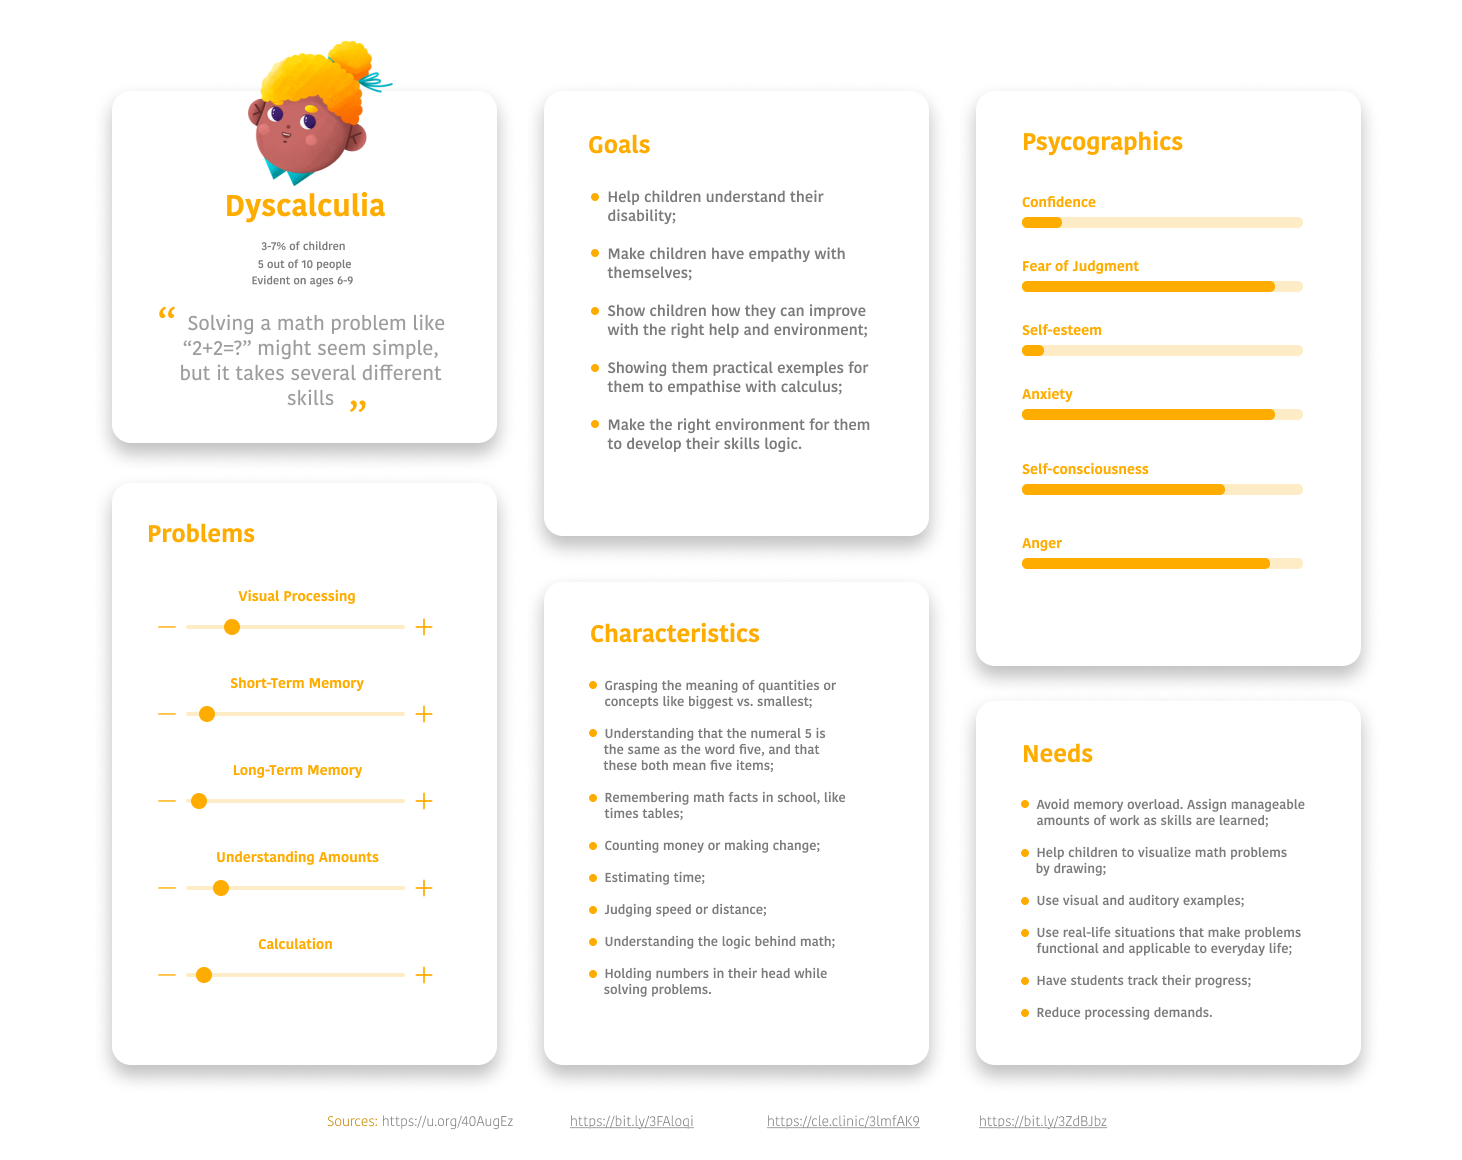
\includegraphics[width=0.8\linewidth]{Chapters/figma/Discalculia.png}
    \caption{Dyscalculia User Profile}
    \label{fig:dyscalculiaUserProfile}
\end{figure}

\paragraph{Goals}
\begin{itemize}
    \item \textbf{Help children understand their disability}: The mini-games aim to provide children with a clear understanding of Dyscalculia, its impact on their mathematical abilities, and how it does not define their overall intelligence.
    \item \textbf{Foster empathy and self-acceptance}: By creating an environment of empathy and self-acceptance, the mini-games aim to help children develop a positive self-image and reduce negative emotions related to their difficulties with mathematics.
    \item \textbf{Show children how they can improve}: The mini-games should demonstrate to children that with the right help, strategies, and environment, they can improve their mathematical skills and overcome challenges associated with Dyscalculia.
    \item \textbf{Provide practical examples for empathy with calculus}: The mini-games can present practical examples or real-life scenarios to help children develop an empathetic understanding of mathematical concepts and their relevance in everyday life.
    \item \textbf{Create an environment for logical skill development}: The mini-games should provide a supportive and stimulating environment for children to develop their logical and mathematical reasoning abilities.
\end{itemize}

\paragraph{Psycographics}
\begin{itemize}
    \item \textbf{Low confidence}: Children with Dyscalculia often struggle with their mathematical abilities, leading to low confidence in their own skills \cite{understood2024}.
    \item \textbf{High fear of judgment}: Due to difficulties with math, children may fear being judged or evaluated negatively by peers or teachers \cite{understood2024}.
    \item \textbf{Low self-esteem}: Struggles with mathematics can negatively impact self-esteem and self-worth \cite{clevelandclinic2024}.
    \item \textbf{High anxiety}: Children with Dyscalculia may experience anxiety or stress when faced with mathematical tasks or assessments \cite{pmc2024}.
    \item \textbf{High self-consciousness}: Difficulties with mathematics can make children self-conscious about their abilities and performance in academic settings \cite{understood2024}.
    \item \textbf{High anger}: Frustration arising from mathematical challenges can lead to feelings of anger or irritability \cite{clevelandclinic2024}.
\end{itemize}

\paragraph{Problems}
\begin{itemize}
    \item \textbf{Visual processing}: Difficulties in processing and interpreting visual information related to numbers, symbols, and mathematical representations \cite{understood2024}.
    \item \textbf{Short/Long-Term memory}: Challenges in retaining and recalling mathematical facts, formulas, and procedures from both immediate and long-term memory \cite{clevelandclinic2024}.
    \item \textbf{Understanding amounts}: Difficulty grasping the concept of quantity, comparing magnitudes, and understanding number relationships \cite{clevelandclinic2024}.
    \item \textbf{Calculation}: Challenges in performing mathematical calculations, such as addition, subtraction, multiplication, and division \cite{understood2024}.
\end{itemize}

\paragraph{Characteristics}
\begin{itemize}
    \item \textbf{Grasping the meaning of quantities or concepts}: Difficulties in understanding concepts such as big versus small, more versus less, or numerical symbols representing quantities \cite{clevelandclinic2024}.
    \item \textbf{Understanding number-word correspondence}: Struggles in connecting numeral symbols with their corresponding written words and comprehending that they both represent the same quantity \cite{understood2024}.
    \item \textbf{Remembering math facts}: Challenges in recalling and memorizing math facts, such as times tables or basic arithmetic operations \cite{clevelandclinic2024}.
    \item \textbf{Counting money or making change}: Difficulties in accurately counting money, making change, or understanding monetary concepts \cite{clevelandclinic2024}.
    \item \textbf{Estimating time}: Trouble estimating and judging the passage of time accurately \cite{understood2024}.
    \item \textbf{Judging speed or distance}: Challenges in assessing speed, distance, or spatial relationships \cite{pmc2024}.
    \item \textbf{Understanding the logic behind math}: Difficulties in comprehending the underlying logic and reasoning behind mathematical concepts and operations \cite{understood2024}.
    \item \textbf{Holding numbers in their head}: Struggles in retaining and manipulating numbers mentally while solving mathematical problems \cite{clevelandclinic2024}.
\end{itemize}

\paragraph{Needs}
\begin{itemize}
    \item \textbf{Avoiding memory overload}: Assigning manageable amounts of work that align with children's learning abilities and gradually increasing the complexity as skills are learned and mastered \cite{clevelandclinic2024}.
    \item \textbf{Visualizing math problems}: Incorporating visual elements and encouraging children to draw or visualize mathematical problems to enhance understanding and problem-solving \cite{understood2024}.
    \item \textbf{Utilizing visual and auditory examples}: Presenting mathematical concepts and problems through visual and auditory means to address different learning modalities and enhance comprehension \cite{pmc2024}.
    \item \textbf{Real-life applications}: Designing mini-games that incorporate real-life situations and practical examples to demonstrate the functional and applicable aspects of mathematical concepts in everyday life \cite{understood2024}.
    \item \textbf{Tracking progress}: Providing mechanisms for children to track their progress and achievements within the mini-games to foster a sense of accomplishment and motivation.
    \item \textbf{Reducing processing demands}: Implementing strategies and adjustments within the mini-games to reduce cognitive processing demands, such as providing additional time, scaffolding instructions, or offering alternative problem-solving approaches \cite{understood2024}.
\end{itemize}
